%%%%%%%%%%%%%%%%%%%%%%%%%%%%%%%%%%%%%%%%%%%%%%%%%%%%%%%%%%%%%%%%%%%%%%%%%%%%%%
% Template LaTeX Template Version 1.0 (December 8 2014)
%
% This template has been downloaded from: http://www.LaTeXTemplates.com
%
% Original author: Brandon Fryslie With extensive modifications by: Vel
% (vel@latextemplates.com)
%
% License: CC BY-NC-SA 3.0 (http://creativecommons.org/licenses/by-nc-sa/3.0/)
%
% Authors: Sabbir Ahmed
% 
%%%%%%%%%%%%%%%%%%%%%%%%%%%%%%%%%%%%%%%%%%%%%%%%%%%%%%%%%%%%%%%%%%%%%%%%%%%%%%

\documentclass[paper=usletter, fontsize=12pt]{article}
%%%%%%%%%%%%%%%%%%%%%%%%%%%%%%%%%%%%%%%%%
% Contract Structural Definitions File Version 1.0 (December 8 2014)
%
% Created by: Vel (vel@latextemplates.com)
% 
% This file has been downloaded from: http://www.LaTeXTemplates.com
%
% License: CC BY-NC-SA 3.0 (http://creativecommons.org/licenses/by-nc-sa/3.0/)
%
%%%%%%%%%%%%%%%%%%%%%%%%%%%%%%%%%%%%%%%%%

\usepackage{geometry} % Required to modify the page layout
\usepackage{multicol}
\usepackage{amsmath}
\usepackage{amssymb}

\usepackage[pdftex]{graphicx}
\usepackage{wrapfig}
\usepackage[font=scriptsize, labelfont=bf]{caption}
\usepackage[utf8]{inputenc} % Required for including letters with accents
\usepackage[T1]{fontenc} % Use 8-bit encoding that has 256 glyphs

\usepackage{avant} % Use the Avantgarde font for headings
\usepackage{courier}
\usepackage{xparse}
\usepackage{xcolor}
\usepackage{listings}  % for code verbatim and console outputs

\setlength{\textwidth}{16cm} % Width of the text on the page
\setlength{\textheight}{23cm} % Height of the text on the page
\setlength{\oddsidemargin}{0cm} % Width of the margin - negative to move text left, positive to move it right
\setlength{\topmargin}{-1.25cm} % Reduce the top margin

\setlength{\parindent}{0mm} % Don't indent paragraphs
\setlength{\parskip}{2.5mm} % Whitespace between paragraphs
\renewcommand{\baselinestretch}{1.5}

\definecolor{green}{rgb}{0.18, 0.55, 0.34}

\graphicspath{ {figures/} }
\captionsetup[table]{skip=10pt}

\lstset{language=C, keywordstyle={\bfseries \color{black}}}

% defines algorithm counter for chapter-level
\newcounter{nalg}[section]

%defines appearance of the algorithm counter
\renewcommand{\thenalg}{\thesection .\arabic{nalg}}

% defines a new caption label as Algorithm x.y
\DeclareCaptionLabelFormat{algocaption}{Algorithm \thenalg}

% defines the algorithm listing environment
\lstnewenvironment{pseudocode}[1][] {
    \refstepcounter{nalg}  % increments algorithm number
    \captionsetup{font=normalsize, labelformat=algocaption, labelsep=colon}
    \lstset{
        breaklines=true,
        mathescape=true,
        numbers=left,
        numberstyle=\scriptsize,
        basicstyle=\footnotesize\ttfamily,
        keywordstyle=\color{black}\bfseries,
        keywords={input, output, return, parallel, function, for, to, in, if,
        else, foreach, while, and, or, new, print},
        xleftmargin=.04\textwidth,
        #1
    }
}{}

\renewcommand{\familydefault}{\sfdefault}  % default font for entire document
 % specifies the document layout and style

\usepackage{array}
\usepackage{multirow}
\usepackage[font=small, labelfont=bf]{caption}
\usepackage{listings}
\lstset{
    mathescape=True
}
\captionsetup[table]{skip=10pt}
\renewcommand{\arraystretch}{1.2}

\begin{document}

    \documentinfo {\textbf{Homework 7: VGA Circle Report}}
    {\today} {Sabbir Ahmed}
    \vspace{-0.1in}

    \section{Background} In this project students will explicitly implement a
    computational finite-state machine, utilize rescheduling and resource
    sharing, and become familiar with the concept of using an on-chip clock
    multiplier. Students will leverage the faster clock to implement
    computations in a serial fashion. In this project, students will display a
    circle on the screen, examine analysis reports, and modify synthesis
    options.

    Before the implementation, the previous VGA rectangle was resynthesized to
    generate its timing report with the newly added Digital Clock Manager
    (DCM). Figure \ref{fig:recttime} provides the clock report generated,
    showing it met the timing constraints.
    \begin{figure}[ht]
        \begin{center}
            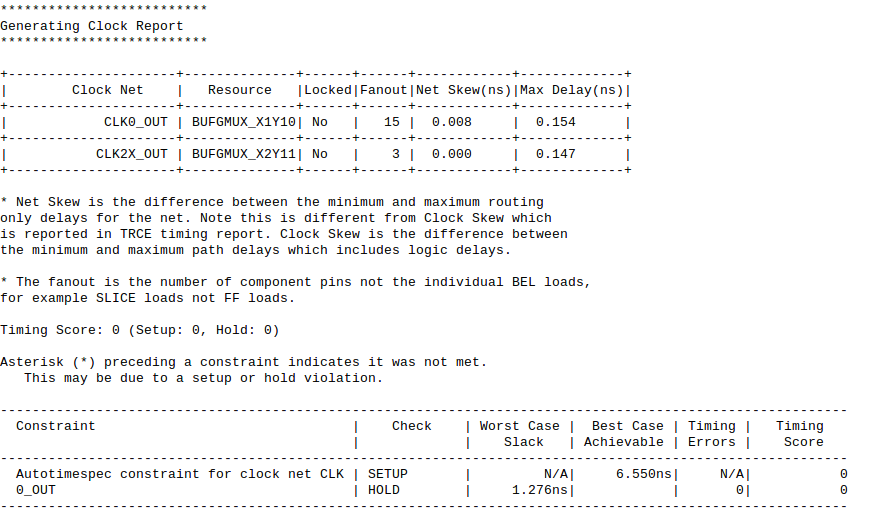
\includegraphics[width=1\textwidth]{recttime.png}
            \caption{Screen capture of the clock report of the rectangle.}
            \label{fig:recttime}
        \end{center}
    \end{figure}

    \section{Implementation} Multiple designs were implemented to analyze their
    effects on resource sharing and timing constraints.

        \subsection{Single Cycle Computation Design} The initial design
        implemented the entire inequality in a single cycle. Since the design
        emphasized on the computation being performed in a single cycle,
        explicitly generating several registers to hold the constant state
        value was unnecessary. An additional state was included for the
        synthesizer to consider encoding the FSM. The single-state module
        successfully generated the circle on the VGA screen using the formula
        $(x - x_c)^2 + (y - y_c)^2 < 10000$. The module is initialized with an
        asynchronous reset.

        \subsubsection{States} Table \ref{table:singlefsmcode} provides the FSM
        states encoded by the synthesizer. The automatic-encoding encoded
        states do not differ from the values assigned to them during
        initialization because of the small number of states. The states were
        intentionally assigned with 2-bit values to alert the synthesizer of
        the FSM.

        \begin{table}[h]
            \caption{FSM state encoding generated by the synthesizer for the
            single cycle design.}
            \label{table:singlefsmcode}
            \centering
            \begin{tabular}{ m{5em}m{5em} }
                \hline
                \textbf{State}  &    \textbf{Encoding} \\
                \hline
                00              &    00 \\
                01              &    01 \\
                \hline
            \end{tabular}
        \end{table}
        \newpage

        \begin{enumerate}

            \item \textbf{INIT (00): } Serves as a buffer to the computational
            state. This state serves no other purpose.

            \item \textbf{COMPUTE (01): } Computes the entire circle
            inequality.

        \end{enumerate}

        \subsubsection{Testbench} Figure \ref{fig:singwav} provides the
        waveforms generated by sample coordinates $(x, y)$ to the module.
        \begin{figure}[ht]
            \begin{center}
                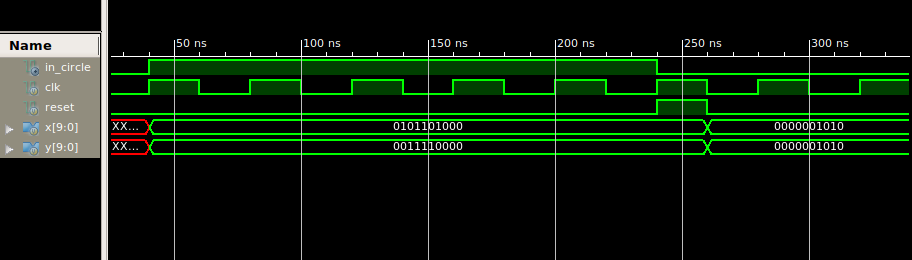
\includegraphics[width=1\textwidth]{singwav.png}
                \caption{Single cycle computation design demonstrating the
                circle flag (\texttt{in\_circle}) activated at $(360, 240)$ and
                deactivated at $(10,10)$.}
                \label{fig:singwav}
            \end{center}
        \end{figure}

        \subsubsection{Synthesis} As expected, the design did not meet the
        timing constraints. Figure \ref{fig:singtime} provides the summary of
        the time constraints report, where the constraint
        \texttt{TS\_uut\_CLK0\_BUF} was not met.

        \begin{figure}[ht]
            \begin{center}
                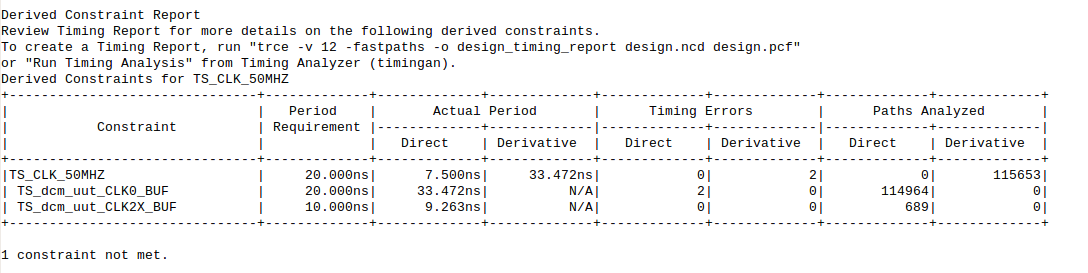
\includegraphics[width=1\textwidth]{singtime.png}
                \caption{Screen capture of the timing constraint report showing
                failure of \texttt{TS\_uut\_CLK0\_BUF} of the DCM.}
                \label{fig:singtime}
            \end{center}
        \end{figure}

        \begin{table}[h]
            \caption{Timing slacks of \texttt{TS\_uut\_CLK0\_BUF}}
            \label{table:singslacks}
            \centering
            \begin{tabular}{ m{5em}m{10em} }
                \hline
                \textbf{Check}  &   \textbf{Worst Case Slack} \\
                \hline
                SETUP           &   -6.736 ns \\
                HOLD            &   1.003 ns \\
                \hline
            \end{tabular}
        \end{table}

        Table \ref{table:singlemacro} provides the macro statistics generated
        by the synthesizer.

        \begin{table}[h]
            \caption{Macro statistics generated by the synthesizer for the
            single cycle design.}
            \label{table:singlemacro}
            \centering

            \begin{tabular*}{250pt}{ m{20em}m{1cm} }
                \textbf{\# Multipliers}         & \textbf{2} \\
                 11x11-bit multiplier           & 2 \\
                \textbf{\# Adders/Subtractors}  & \textbf{4} \\
                 10-bit adder                   & 1 \\
                 11-bit subtractor              & 2 \\
                 23-bit adder                   & 1 \\
                \textbf{\# Counters}            & \textbf{2} \\
                 10-bit up counter              & 2 \\
                \textbf{\# Registers}           & \textbf{8} \\
                 1-bit register                 & 8 \\
                \textbf{\# Comparators}         & \textbf{1} \\
                 24-bit comparator less         & 1 \\
            \end{tabular*}

        \end{table}

        The multipliers are used to multiply the two 10-bit coordinates.
        Several adders and subtractors are used in the design to handle
        \texttt{pos\_v}, \texttt{pos\_h} and the center coordinates.

        \subsubsection{Files} The design for the single cycle computation was
        modularized and implemented as a standalone top-level design. The file
        is provided as \texttt{top\_single\_cycle.v} which utilizes the single
        cycle modules exclusively.

        \subsection{Multiple Cycle Computation Design with Resource Sharing}
        The multiple cycles design distributed the computations over multiple
        cycles in multiple states. The design utilized 4 states to compute the
        circle inequality. Since this design accumulated its final output over
        multiple cycles, several registers had to be initialized with
        sufficient capabilities. Since the coordinates are 10-bits in size,
        their highest decimal value is $2^{10}-1=1023$. Squaring that integer
        would result in a 20-bit number. Therefore, temporary registers of
        20-bits were allocated to hold values for the computation.

        \subsubsection{States} Table \ref{table:multifsmcode} provides the FSM
        states encoded by the synthesizer. The synthesizer encoded the states
        with one-hot encoding, differing from the binary values initialized to
        them.

        \begin{table}[h]
            \caption{FSM state encoding generated by the synthesizer for the
            multiple cycle design.}
            \label{table:multifsmcode}
            \centering
            \begin{tabular}{ m{5em}m{5em} }
                \hline
                \textbf{State}  &   \textbf{Encoding} \\
                \hline
                00              &   0001 \\
                01              &   0010 \\
                10              &   0100 \\
                11              &   1000 \\
                \hline
            \end{tabular}
        \end{table}

        \begin{enumerate}

            \item \textbf{INIT (0001): } Subtracts the coordinates from the
            corresponding center coordinates. Parameters \texttt{XLEFT} of
            value 320 and \texttt{YBOTTOM} of value 240 were used as the center
            coordinates of a standard VGA monitor.

            \item \textbf{SQUAREX (0010): } Multiplies the $x$ coordinate with
            itself, and stores it in the temporary \texttt{mul\_temp}.

            \item \textbf{SQUAREY (0100): } Stores the previous value of
            \texttt{mul\_temp} to a different variable \texttt{x\_temp}.
            Multiplies the $y$ coordinate with itself, and stores it in the
            temporary \texttt{mul\_temp}.

            \item \textbf{ADDCMP (1000): } Adds \texttt{mul\_temp} to
            \texttt{x\_temp}, and then compares with the radius. This
            comparison generates a 1-bit signal for the circle flag,
            terminating the computation.

        \end{enumerate}

        \subsubsection{Testbench} Figure \ref{fig:singwav} provides the
        waveforms generated by sample coordinates $(x, y)$ to the module.
        \begin{figure}[ht]
            \begin{center}
                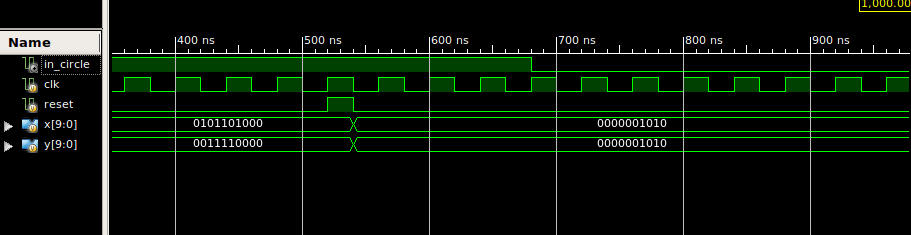
\includegraphics[width=1\textwidth]{multiwav.png}
                \caption{Multiple cycle computation design demonstrating the
                circle flag (\texttt{in\_circle}) activated at $(360, 240)$ and
                deactivated at $(10,10)$.}
                \label{fig:multiwav}
            \end{center}
        \end{figure}

        \subsubsection{Synthesis} The design successfully synthesized while
        meeting the timing constraints. The \texttt{``All constraints were
        met.''} line was seen in the timing report. Figure \ref{fig:singtime}
        provides the summary of the time constraints report.

        \begin{figure}[ht]
            \begin{center}
                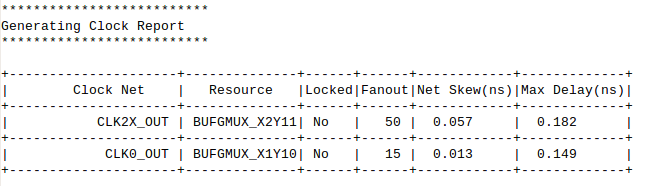
\includegraphics[width=1\textwidth]{multiclk.png}
                \caption{Screen capture of the timing constraint report showing
                the multiple cycle design meeting all timing constraints.}
                \label{fig:multiclk}
            \end{center}
        \end{figure}

        \begin{table}[h]
            \caption{Timing slacks for each clock domains.}
            \label{table:singslacks}
            \centering
            \begin{tabular}{ lm{5em}m{10em} }
\hline
\textbf{Constraint} & \textbf{Check}  &   \textbf{Worst Case Slack} \\
\hline
\multirow{ 2}{*}{Autotimespec constraint for clock net CLK2X\_OUT} & SETUP &
N/A \\
 & HOLD & 1.017ns \\
\multirow{ 2}{*}{Autotimespec constraint for clock net CLK0\_OUT} & SETUP &
N/A \\
 & HOLD & 1.200ns \\

\hline
            \end{tabular}
        \end{table}

        In terms of resource sharing, the design utilized a single multiplier
        as intended. Table \ref{table:multimacro} provides the macro statistics
        generated by the synthesizer.

        \begin{table}[h]
            \caption{Macro statistics generated by the synthesizer for the
            multi cycle design.}
            \label{table:multimacro}
            \centering
            \begin{tabular*}{250pt}{ m{20em}m{1cm} }
            \textbf{\# Multipliers}         & \textbf{1} \\
             20x20-bit multiplier           & 1 \\
            \textbf{\# Adders/Subtractors}  & \textbf{4} \\
             10-bit adder                   & 1 \\
             10-bit subtractor              & 1 \\
             12-bit subtractor              & 1 \\
             21-bit adder                   & 1 \\
            \textbf{\# Counters}            & \textbf{2} \\
             10-bit up counter              & 2 \\
            \textbf{\# Registers}           & \textbf{11} \\
             1-bit register                 & 8 \\
             10-bit register                & 1 \\
             20-bit register                & 2 \\
            \textbf{\# Comparators}         & \textbf{1} \\
             22-bit comparator less         & 1 \\
            \end{tabular*}

        \end{table}
        \newpage

        \subsection{Multiple Cycle Computation Design without Resource Sharing}
        The design for this multiple cycles implementation is identical to the
        multiple cycles design with resource sharing. There is no difference in
        the macro statistics when the \texttt{-resource\_sharing} is turned
        off.

        \begin{table}[h]
            \caption{Macro statistics generated by the synthesizer for the
            multi cycle design without resource sharing.}
            \label{table:multimacro}
            \centering
            \begin{tabular*}{250pt}{ m{20em}m{1cm} }
            \textbf{\# Multipliers}         & \textbf{1} \\
             20x20-bit multiplier           & 1 \\
            \textbf{\# Adders/Subtractors}  & \textbf{4} \\
             10-bit adder                   & 1 \\
             10-bit subtractor              & 1 \\
             12-bit subtractor              & 1 \\
             21-bit adder                   & 1 \\
            \textbf{\# Counters}            & \textbf{2} \\
             10-bit up counter              & 2 \\
            \textbf{\# Registers}           & \textbf{11} \\
             1-bit register                 & 8 \\
             10-bit register                & 1 \\
             20-bit register                & 2 \\
            \textbf{\# Comparators}         & \textbf{1} \\
             22-bit comparator less         & 1 \\
            \end{tabular*}

        \end{table}

\newpage
\section{Listings}
\begin{lstlisting}[language=Verilog, caption=Single Cycle Computation State Machine]
always @(posedge clk) begin
    if (reset) begin
        in_circle <= 0;
        state <= INIT;
    end else begin
        case (state)
            INIT: begin
                state <= COMPUTE;
            end
            COMPUTE: begin
                // (x - x$_C$)$^2$ + (y - y$_C$)$^2$ < 10000
                in_circle <= (
                    ((x - XLEFT) * (x - XLEFT) +    // (x - x$_C$)$^2$ +
                    (y - YBOTTOM) * (y - YBOTTOM))  // (y - y$_C$)$^2$
                    < RADIUS                        // < 10000
                );
                state <= INIT;
            end
        endcase
    end
end
\end{lstlisting}


\end{document}
